%%%%%%%%%%%%%%%%%%%%%%%%%%%%%%%%%%%%%%%%%%%%%%%%%%%%%%%%%%%%%%%%%%%%%%%%%%%%%%%%%%%%%%%%%%%%%%%%%%%
% Chapter 5 -> Parameter Refinements
% Author: Eduardo G Gusmao
%%%%%%%%%%%%%%%%%%%%%%%%%%%%%%%%%%%%%%%%%%%%%%%%%%%%%%%%%%%%%%%%%%%%%%%%%%%%%%%%%%%%%%%%%%%%%%%%%%%
\chapter{Parameter Refinements}
\label{cha:parameter.refinements}

\graphicspath{{chapter5/figs/}}

% Introduction
In this chapter we justify the selection of specific parameters on the creation or execution of: signal treatment strategies (Section~\ref{sec:signal.parameterization}), the hidden Markov model method (Section~\ref{sec:hmm.parameterization}), the signal filtering method (Section~\ref{sec:filters.parameterization}), method evaluation methodologies (Section~\ref{sec:evaluation.methodology.parameterization}) and competing methods (Section~\ref{sec:competing.methods.parameterization}). The chapter closes with a few concluding remarks on the importance of such parameter selection experiments (Section~\ref{sec:conclusion.5}).

All parameter selection experiments described in this chapter were based on data from the {\tt Comprehensive} ChIP-seq evaluation data set (with exception of Section~\ref{sec:flrexp.footprint.quality.score}, in which FLR-Exp was obviously used). All parameter selection that involved the performance evaluation of HINT was performed using the model with DNase $+$ H3K4me1 $+$ H4K4me3. All analyses on competing methods used the {\tt Benchmarking} ChIP-seq evaluation data set. All experiments were performed only on data from human chromosome~1 (full length $= 249,250,621$ bp), which was removed from all further method comparison analyses.

%%%%%%%%%%%%%%%%%%%%%%%%%%%%%%%%%%%%%%%%%%%%%%%%%%%%%%%%%%%%%%%%%%%%%
% Section: Signal Parameterization
%%%%%%%%%%%%%%%%%%%%%%%%%%%%%%%%%%%%%%%%%%%%%%%%%%%%%%%%%%%%%%%%%%%%%
\section{Signal Parameterization}
\label{sec:signal.parameterization}

%Although the first normalization step (within-dataset) is always used in a local fashion~\cite{boyle2011}, the second normalization step, i.e. the scaling procedure, can be performed using either local or global values of the standard deviation and percentile. The local method is depicted in Equation~\ref{xxx}, using the same windowing as the normalization procedure. The global method consists on using a single estimate of standard deviation and percentile for each cell type.

We have performed an empirical analysis to drive the choice of the scaling methodology and to test different percentile cutoffs. We created ROC curves and calculated their AUCs using HINT with signals generated with either global or local methodologies combined with either the $96^{th}$, $98^{th}$ or $99^{th}$ percentiles.

We have created boxplots with the distribution of the differences between the local and global scaling approaches (Figure~\ref{fig:gusmao_signal_parameterization}a) and between the different percentiles tested (Figure~\ref{fig:gusmao_signal_parameterization}b). The distributions show a slight advantage for the local approach and for higher percentile values. Concerning the choice of percentile, both $98^{th}$ and $99^{th}$ percentiles are superior to the $96^{th}$ percentile. We chose to use $98^{th}$ percentile as it presents a more lenient criteria. Strict parameters usually lead to overfitting and AUC results can be misleading for specificity-overfitted methods. The choice of a lenient percentile was made in order to present a more fair comparison landscape.

Loosely speaking, using the $98^{th}$ percentile means that only the top $2\%$ values will have a value greater than $0.5$, since the scaling follows a logistic function. This is supported by estimates of the average coverage of DHSs or regions enriched with histone marks over multiple cell types in the human genome~\cite{encode2012} (see Supplementary Table~\ref{tab:coverage}). The Supplementary Figure~\ref{fig:gusmao_signal_parameterization} shows examples of normalized and slope signals using the selected scaling parameters.

% Figure - Signal parameterization
\begin{figure}[h!]
\centering
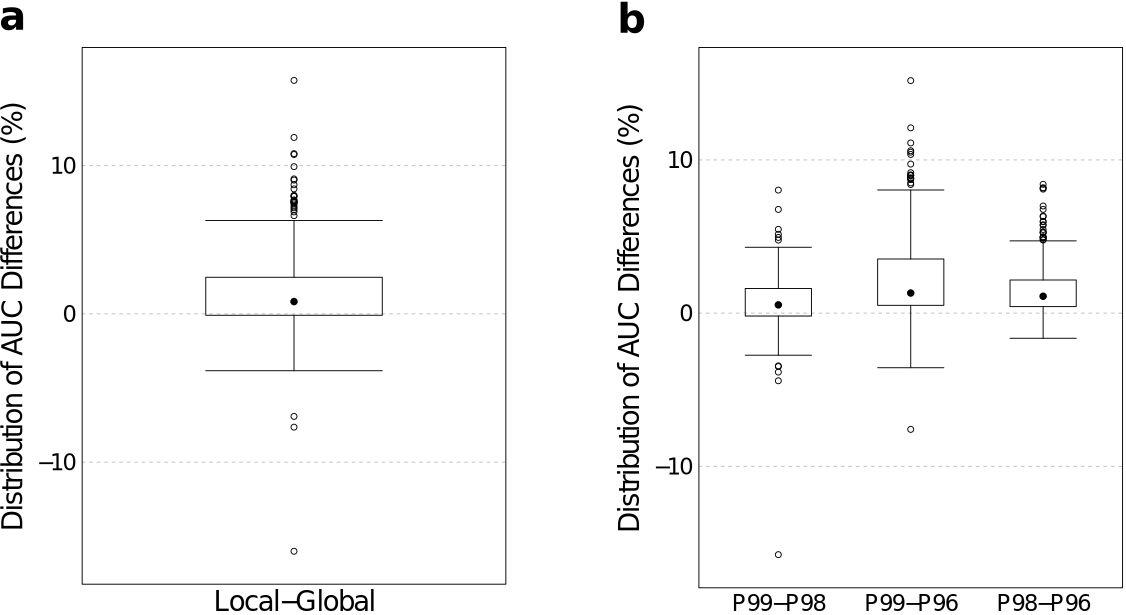
\includegraphics[width=0.80\textwidth]{gusmao_signal_parameterization}
\caption[Signal parameterization]{\textbf{Signal parameterization.} (\textbf{a}) Distribution of the difference between local and global AUCs for all percentile values tested. Positive values indicate the advantage of the local approach. (\textbf{b}) Distribution of the difference between specific percentile values given the local approach. Positive values indicate the advantage of higher percentiles.}
\label{fig:gusmao_signal_parameterization}
\end{figure}

%%%%%%%%%%%%%%%%%%%%%%%%%%%%%%%%%%%%%%%%%%%%%%%%%%%%%%%%%%%%%%%%%%%%%
% Section: Hidden Markov Model Parameterization
%%%%%%%%%%%%%%%%%%%%%%%%%%%%%%%%%%%%%%%%%%%%%%%%%%%%%%%%%%%%%%%%%%%%%
\section{Hidden Markov Model Parameterization}
\label{sec:hmm.parameterization}

% Introduction
In this section we explore some variations of the hidden Markov model topology (Section~\ref{sec:alternative.topologies}). Furthermore, we analyze empirically the usage of the two main decoding algorithms (Section~\ref{sec:impact.different.decoding.algorithms}).

% TODO - usar essa parte
We have performed a set of experiments to evaluate/justify methodological choices for our
approach. For this, we used the genomic signals of chromosome~1, which was left out of any
further analysis. First, we evaluated choices of scaling parameters: use of global or local
statistics in Eq.~\ref{eq:norm2} and value of the percentile (96$\%$, 98$\%$ and 99$\%$).
Results indicate the advantage of local normalization and that 98$\%$ was a good trade-off
between sensitivity and specificity. We have also compared the use of the Viterbi algorithm
and posterior decoding to detect the footprints. Experimental results indicate a slight
advantage of the Viterbi algorithm, while the posterior decoding had numerical problems
in particular genomic regions. We have also evaluated two distinct HMM topologies. The first
alternative merges {\tt UP}--{\tt TOP}--{\tt DOWN} states in one to obtain a simple HMM. This HMM has
very poor performance, as it does not take advantage of the slope of the DHS/histone modification signals.
We have also extended the original HMM topology by including transitions from the background
states directly to the DNase level states. This modification allows the detection of DHS peaks
between asymmetric histone modification signals, which were evidenced in~\cite{kundaje2012}.
The HMM had smaller AUC values than the HMM model proposed here and was therefore not
explored. See Supplementary Section~3 for further discussion regarding all empirical
analyses on HMM parameter selection. All HMMs were implemented using Scikit~\cite{pedregosa2011}.
All experiments were executed in 4 Xeon E7-4870 CPUs with 10 2.4GHz cores each.
%%%%%%%%%%%%%%%%%%%%%

%%%%%%%%%%%%%%%%%%%%%%%%%%%%%%%%%%%%%%%%%%%%%%%%%%%%%%%%%%%%%%%%%%%%%
% Section: Alternative Topologies
%%%%%%%%%%%%%%%%%%%%%%%%%%%%%%%%%%%%%%%%%%%%%%%%%%%%%%%%%%%%%%%%%%%%%
\subsection{Alternative Topologies}
\label{sec:alternative.topologies}

The individual pattern of DNase-seq around active TFBSs generally follows the peak-dip-peak trend when we consider aligned reads from both strands. This follows directly from the DNase-seq protocol, wherein the DNase I enzyme nicks the DNA in loci that can be reached~\cite{crawford2006b,song2010,boyle2011} (see Section~\ref{xxx}). However, although the average histone modifications trend generally presents a very clear (close to symmetric) peak-dip-peak pattern, there is inherent heterogeneity within individual \emph{loci} regarding signal magnitude, asymmetry and implicit strand orientation~\cite{kundaje2012,encode2012}. In other words, Kundaje et al.~\cite{kundaje2012} showed that part of the histone modification ChIP-seq signal does not present a symmetric peak-dip-peak pattern, which might impact on the performance of HINT when histone modifications are used.

We have therefore evaluated two additional HMM topologies depicted in Figure~\ref{fig:gusmao_alternative_topologies}. The model M2 (Figure~\ref{fig:gusmao_alternative_topologies}b) is an extension of the original model (here denoted as M1; Figure~\ref{fig:gusmao_alternative_topologies}a) to account for the histone modification signal asymmetry, i.e. that some DHSs have very small signals of active histone modifications on its downstream or upstream regions. For such, two additional transitions were added (shown in red in Figure~\ref{fig:gusmao_alternative_topologies}b) in order to allow the DNase level states to be visited when there are no histone modification peaks before or after DNase-seq peaks. The new transition probabilities were estimated taking into account the proportions of asymmetrical peaks reported in Kundaje et al.~\cite{kundaje2012}. The model M3 (Figure~\ref{fig:gusmao_alternative_topologies}c) is a simplification of M1, which performs the predictions of footprints without the slope signal. In M3, the {\tt UP}, {\tt TOP} and {\tt DOWN} states from M1 are compressed into one state -- {\tt HIGH} -- which recognizes high levels of DNase-seq cleavage activity (DNase level state) or high levels of histone modifications (histone level state). Consequently, the HMM needs only the normalized signal and becomes bivariate (DNase-seq and histone modifications normalized signals).

% Figure - Alternative HMM topologies
\begin{figure}[h!]
\centering
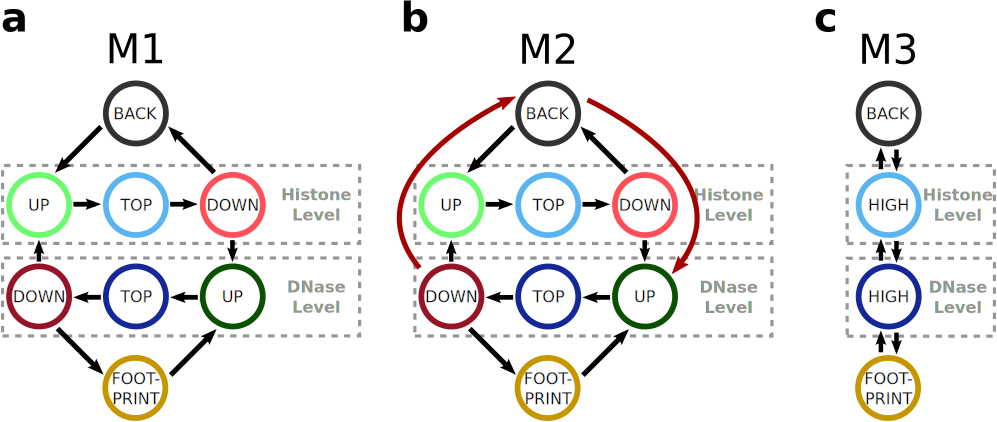
\includegraphics[width=0.99\textwidth]{gusmao_alternative_topologies}
\caption[Alternative HMM topologies]{\textbf{Alternative HMM topologies.} (\textbf{a}) Original model that captures the TFBS grammar. Here, we call this model M1. (\textbf{b}) Alternative model to account for histone modification heterogeneity. Here, we call this model M2. (\textbf{c}) Alternative model that proposes a simpler solution than the original method M1. Here, we call this model M3.}
\label{fig:gusmao_alternative_topologies}
\end{figure}

We tested these three models and measured their performance (AUC). The Figure~\ref{fig:gusmao_alternative_topologies_results} shows the distribution of the AUC differences between these models. We observe a slight advantage for M1 when compared to M2 ($p$-value $ < 10^{-20} $) and a clear advantage of M1 and M2 over M3 ($p$-value $ < 10^{-58} $ and $ < 10^{-37} $, respectively).

The possible reason for the good results of M1 in relation to M2 is the fact that the normalization methodology emphasizes even little increases in histone levels leveraging the asymmetry issue (see Supplementary Figure~\ref{fig:asymmetric}). Furthermore, the poor performance of M3 in comparison to M1 and M2 indicates that even with more complex models (4 \emph{versus} 2 variables and 8 \emph{versus} 4 states, respectively) the slope signal and the additional states are crucial in the accurate delineation of the footprints.

% Figure - Accuracy of alternative HMM topologies
\begin{figure}[h!]
\centering
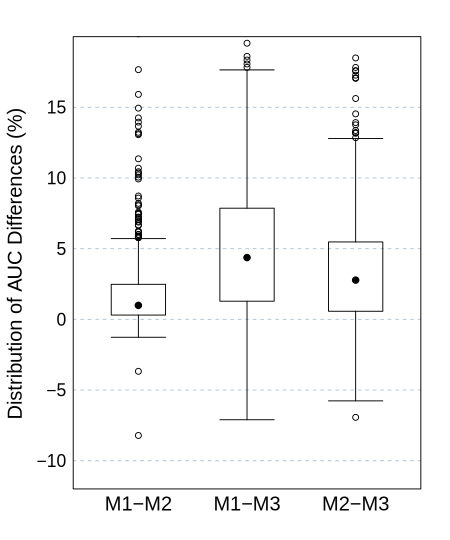
\includegraphics[width=0.99\textwidth]{gusmao_alternative_topologies_results}
\caption[Accuracy of alternative HMM topologies]{\textbf{Accuracy of alternative HMM topologies.} Distribution of AUC differences between all HMM topologies tested (M1, M2 and M3). We are able to observe a significant advantage towards the model M1 ($p$-value $10^{-20}$). Therefore, the model M1 is going to be used in all further analyses.}
\label{fig:gusmao_alternative_topologies_results}
\end{figure}

%%%%%%%%%%%%%%%%%%%%%%%%%%%%%%%%%%%%%%%%%%%%%%%%%%%%%%%%%%%%%%%%%%%%%
% Section: Impact of Different Decoding Algorithms
%%%%%%%%%%%%%%%%%%%%%%%%%%%%%%%%%%%%%%%%%%%%%%%%%%%%%%%%%%%%%%%%%%%%%
\subsection{Impact of Different Decoding Algorithms}
\label{sec:impact.different.decoding.algorithms}

In addition to the Viterbi algorithm implementation (see Section~\ref{xxx}), we have tested the usage of posterior decoding~\cite{rabiner1989} (see Section~\ref{xxx}) in order to generate our footprint predictions. In this case, we assume that footprints are contiguous genomic coordinates (represented by $j$) with
\begin{align}
  P(q_{j} = F \! P \: | \: \mathbf{X}) > P(q_{j} = u \: | \: \mathbf{X}) \; \; \; \; \forall \; \; \; u \neq F \! P,
  \label{eq:posterior}
\end{align}
where $ \mathbf{X} $ is the matrix containing the observations (genomic signal) and
$F \! P$ represents the {\tt FOOTPRINT} state.

We show in Figure~\ref{fig:gusmao_alternative_decoding}a the distribution of the pairwise AUC difference between predictions generated using the Viterbi method and posterior decoding. We are able to observe that there is a slight advantage in using the Viterbi method. Despite the lower AUCs for the posterior decoding, one advantage of such technique would be to use the HMM posterior probabilities as priors during operations such as motif matching (similarly as in~\cite{cuellar2012}). However, as can be seen in Figure~\ref{fig:gusmao_alternative_decoding}b, the posterior probability of the HMM being in the {\tt FOOTPRINT} state changes drastically from 0 to 1. Such ``spiky'' distribution confirms that the posterior probability decoding algorithm is not suited for this problem, given the current signal modelling. Therefore, we did not further explore this strategy, opting for the simpler Viterbi approach.

% Figure - Accuracy of different HMM decoding algorithms
\begin{figure}[h!]
\centering
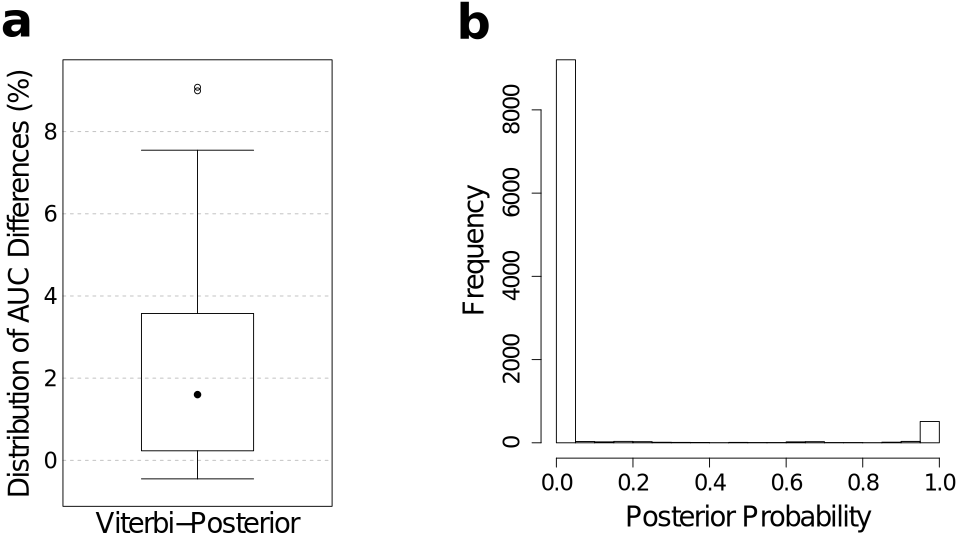
\includegraphics[width=0.99\textwidth]{gusmao_alternative_decoding}
\caption[Accuracy of different HMM decoding algorithms]{\textbf{Accuracy of different HMM decoding algorithms.} (\textbf{a}) Distribution of AUC differences between the predictions made using the Viterbi algorithm and the posterior probability. (\textbf{b}) Distribution of the posterior probability of the HMM being in the state {\tt FOOTPRINT} evaluated in a DHS region in chromosome 1 from 211,431,582 to 211,434,492 bp.}
\label{fig:gusmao_alternative_decoding}
\end{figure}

%%%%%%%%%%%%%%%%%%%%%%%%%%%%%%%%%%%%%%%%%%%%%%%%%%%%%%%%%%%%%%%%%%%%%
% Section: Filters Parameterization
%%%%%%%%%%%%%%%%%%%%%%%%%%%%%%%%%%%%%%%%%%%%%%%%%%%%%%%%%%%%%%%%%%%%%
\section{Filters Parameterization}
\label{sec:filters.parameterization}

Placeholder
% TODO

%%%%%%%%%%%%%%%%%%%%%%%%%%%%%%%%%%%%%%%%%%%%%%%%%%%%%%%%%%%%%%%%%%%%%
% Section: Evaluation Methodology Parameterization
%%%%%%%%%%%%%%%%%%%%%%%%%%%%%%%%%%%%%%%%%%%%%%%%%%%%%%%%%%%%%%%%%%%%%
\section{Evaluation Methodology Parameterization}
\label{sec:evaluation.methodology.parameterization}

% Introduction
We now focus on some choices made regarding parameters used to create the method evaluation techniques. We discuss how we maximized the overlap between MPBSs and TF ChIP-seq peaks while mantaining the computational complexity in a feasible level (Section~\ref{sec:motif.match.bitscore.threshold}). Furthermore, we justify the selection of FLR as the footprint quality score in the FLR-Exp evaluation technique (Section~\ref{sec:flrexp.footprint.quality.score}).

%%%%%%%%%%%%%%%%%%%%%%%%%%%%%%%%%%%%%%%%%%%%%%%%%%%%%%%%%%%%%%%%%%%%%
% Section: Motif Match Bit-Score Threshold
%%%%%%%%%%%%%%%%%%%%%%%%%%%%%%%%%%%%%%%%%%%%%%%%%%%%%%%%%%%%%%%%%%%%%
\subsection{Motif Match Bit-Score Threshold}
\label{sec:motif.match.bitscore.threshold}

We evaluated the use of a fixed bit-score as proposed in~\cite{pique2011} and a dynamic False Positive Rate (FPR)-based criteria~\cite{wilczynski2009}. The latter uses an approach in which the distribution of all possible bit-scores for motifs with the same length as the PFM is evaluated using an optimized algorithm based on dynamic programming to detect significant TFBSs. Then a bit-score cutoff threshold is evaluated based on the value within the PFM-specific bit-score distribution which matches a particular FPR. In the dynamic FPR-based approach, a different threshold is calculated for each TF; while in the fixed bit-score approach, the same cutoff is stablished for all TFs.

In the fixed bit-score approach we used the value proposed by Pique-Regi et al.~\cite{pique2011} of $ log_2(10^4) \approx 13.2877 $. In the dynamic FPR-based approach we tested a FPR of $10^{-4}$. We observed that a more strict FPR ($10^{-5}$) produces results which are equivalent to the fixed bit-score approach and that more a lenient FPR ($10^{-3}$) generates a massive number of MPBSs, increasing the computational complexity to unfeasible levels.

The Table~\ref{xxx} show statistics on the number of MPBSs, ChIP-seq peaks and combinations of both, for K562 cell type. Results regarding other cells can be found in Supplementary Tables~\ref{xxx}--~\ref{xxx}. The fixed bit-score approach (bit-score $= 13.2877 $) is shown always in the top line for each TF; while the varying bit-score at each TF's bottom line correspond to the fynamic FPR-based approach. In all cases, the dynamic FPR-based selection criterion results in a greater proportion of ChIP-seq peaks with an underlying MPBS than the fixed bit-score approach. For instance, only $17.54\%$ of the GABPA peaks in cell type K562 contain overlapping MPBSs selected using bit-score approach, while $37.61\%$ of these peaks contain overlapping MPBSs selected using the FPR-based selection. Therefore, we preferred to use the FPR-based approach, as the fixed bit-score approach represented overly conservative predictions (on average, only $27.71\%$ of the peaks had their corresponding motifs).

% Table - K562 table of mpbs chip statistics (merge part 1 and 2 of bioinfo sup)
% TODO

%%%%%%%%%%%%%%%%%%%%%%%%%%%%%%%%%%%%%%%%%%%%%%%%%%%%%%%%%%%%%%%%%%%%%
% Section: FLR-Exp Footprint Quality Score
%%%%%%%%%%%%%%%%%%%%%%%%%%%%%%%%%%%%%%%%%%%%%%%%%%%%%%%%%%%%%%%%%%%%%
\subsection{FLR-Exp Footprint Quality Score}
\label{sec:flrexp.footprint.quality.score}

As mentioned in Section~\ref{xxx} we evaluated the footprint likelihood ratio (FLR)~\cite{xxx}, footprint score FS~\cite{xxxx} and tag count TC~\cite{xxxx} as footprint quality scores in the FLR-Exp evaluation procedure. The Figure~\ref{gusmao_flrexp_quality_score} exhibits the correlation values obtained when using these footprint quality scores in a set of selected computational footprinting methods.

By observing this Figure~\ref{gusmao_flrexp_quality_score} we are able to see that the FLR metric have superior performance when compared to FS and TC. When considering all methods used in this study, the average correlation values are: FLR $r = xxx$; FS $r = xxx$ and TC $r = xxx$. However, although FLR and FS distributions of correlation metrics differ significantly ($p$-value < $10^{-3}$) the FS provided a very close performance to that of FLR. Therefore, in the absence of the proper computational tools to compute the FLR metric provided by , which is considerably complex; one can use the FS metric in a comparison study without great impact on interpretation. However, in this study we used the FLR statistic as footprint quality score; thus naming this approach FLR-Exp.

% Figure - FLR-Exp results for different footprint quality metrics
\begin{figure}[h!]
\centering

\includegraphics[width=0.99\textwidth]{gusmao_flrexp_quality_score}
\caption[FLR-Exp results for different footprint quality metrics]{\textbf{FLR-Exp results for different footprint quality metrics.} Correlation between Kolmogorov-Smirnov (KS) test statistics versus expression fold change for cell type pair H1- hESC versus K562 by evaluating either the FLR (left), FS (middle) and TC (right) as quality metric for the footprints. Footprints were predicted with HINT-BC, DNase2TF, Neph and FLR (from top to bottom, respectively). The use of FLR as quality metric presents the highest Spearman correlation values (FLR-Exp). On the other hand, TC exhibits small correlation values ($r$ < 0.4) and presents several cases in which the signal of KS and fold change disagree (off diagonal points). Note that the use of FS also have a high average correlation with fold change expression on all evaluated data/methods (average $r$ = 0.73) and indicates a ranking of footprint methods similar to FLR ($r$ = 0.89). Therefore, FS can be used as an alternative to the FLR score as a footprint quality metric.}
\label{fig:gusmao_flrexp_quality_score}
\end{figure}

%%%%%%%%%%%%%%%%%%%%%%%%%%%%%%%%%%%%%%%%%%%%%%%%%%%%%%%%%%%%%%%%%%%%%
% Section: Competing Methods Parameterization
%%%%%%%%%%%%%%%%%%%%%%%%%%%%%%%%%%%%%%%%%%%%%%%%%%%%%%%%%%%%%%%%%%%%%
\section{Competing Methods Parameterization}
\label{sec:competing.methods.parameterization}

% Introduction
In this section we analyze parameter choices for two competing methods: Centipede\cite{pique2011} (Section~\ref{sec:centipede.parameterization}) and Cuellar\cite{cuellar2012} (Section~\ref{sec:cuellar.parameterization}). All other competing methods were either not highly impacted by different parameter choices or the analyses regarding parameter selection were already performed in the original studies.

%%%%%%%%%%%%%%%%%%%%%%%%%%%%%%%%%%%%%%%%%%%%%%%%%%%%%%%%%%%%%%%%%%%%%
% Section: Centipede Parameterization
%%%%%%%%%%%%%%%%%%%%%%%%%%%%%%%%%%%%%%%%%%%%%%%%%%%%%%%%%%%%%%%%%%%%%
\subsection{Centipede Parameterization}
\label{sec:centipede.parameterization}

We have noticed that Centipede was very sensitive to the level of shrinkage of multinomial and negative binomial parameters on a TF- and cell-specific way. The Figure~\ref{fig:gusmao_centipede_roc} shows examples of AUC variation by varying the level of shrinkage of multinomial and negative binomial parameters from $ 0.0 $ to $ 1.0 $ by $ 0.5 $ steps. We observe high AUC changes, in the same parameter settings, when Centipede is applied to distinct TFs. For instance, when the level of shrinkage of multinomial parameters (here abbreviated as $L$) is set to $0.5$ and the level of shrinkage of negative binomial parameters (here abbreviated as $N$) is set to $0.0$ we observe optimal results for the TFs CTCF and GABPA in cell type H1-hESC and for TFs CCNT2 and GATA2 in cell type K562. However, for the same parameters, we observe very low AUCs for TFs Myc and SRF in cell type H1-hESC and for TFs NF-E2 and TBP in cell type K562. In another example, when $L$ is set to $1.0$ and $N$ is set to $0.0$, we observe the best AUC for TFs NF-E2 and TBP but the worst AUC for CCNT2, in cell type K562. Unfortunately, Centipede framework does not provide a procedure for defining such parameters.

Therefore, we decided to perform three evaluation scenarios for Centipede in order to select the best set of parameters in a fair manner. The first uses the default parameters sugested in~\cite{pique2011}, which corresponds to $L = N = 0.0$ (termed `Default'). The second and third scenarios uses $L$ and $N$ parameters estimated in a subset of our gold standard, which includes a random sample of $S$ true MPBSs and $S$ false MPBSs for each TF, where $S$ is the total number of true MPBSs in chromosome~1. In both scenarios, $25$ AUCs are calculated for each TF corresponding to a grid search consisting on the variation of both $L$ and $N$ parameters from $ 0.0 $ to $ 1.0 $ by $ 0.25 $ intervals. In the second scenario, termed `Estimated', we use the grid test results (AUCs) to perform a Friedman-Nemenyi hypothesis test for each cell type in order to estimate the best parameters. Then, we use the parameters estimated in the cell type K562 for the predictions made in cell type H1-hESC and vice versa. In the third scenario, termed `Optimistic', we simply use, for each TF, the parameter settings that generated the best AUC. It is important to point out that this last TF- and cell-specific selection criterion is not applicable on a real scenario, where ChIP-seq experiments for the tested TFs are not available. This was performed only to obtain the method accuracies' upper boundaries for comparison purposes.

The Figure~\ref{fig:gusmao_centipede_test} shows the AUC distribution based on all three scenarios discussed previously. In both cell types, the `Default' model performed poorly than the other two. Also, we observe that the `Estimated' model AUC distribution is close, but still significantly lower than the `Optimistic' model AUC distribution ($p$-value $< 10^{-5}$). Interestingly, the set of parameters estimated in the cell-specific procedure were quite similar ($L=0.75$ and $N=0$ for H1-hESC and $L=0.75$ and $N=0.25$ for K562). Our interpretation is that given our large evaluation set (about 5 times more TFs than in Pique-Regi et al.\cite{pique2011}), these parameter choices are more robust and should be used as default parameters to Centipede. In this study, we will use the `Estimated' scenario since its the best method between both real-case scenarios (`Estimated' and `Default').

% Figure - Centipede AUC variation
\begin{figure}[h!]
\centering
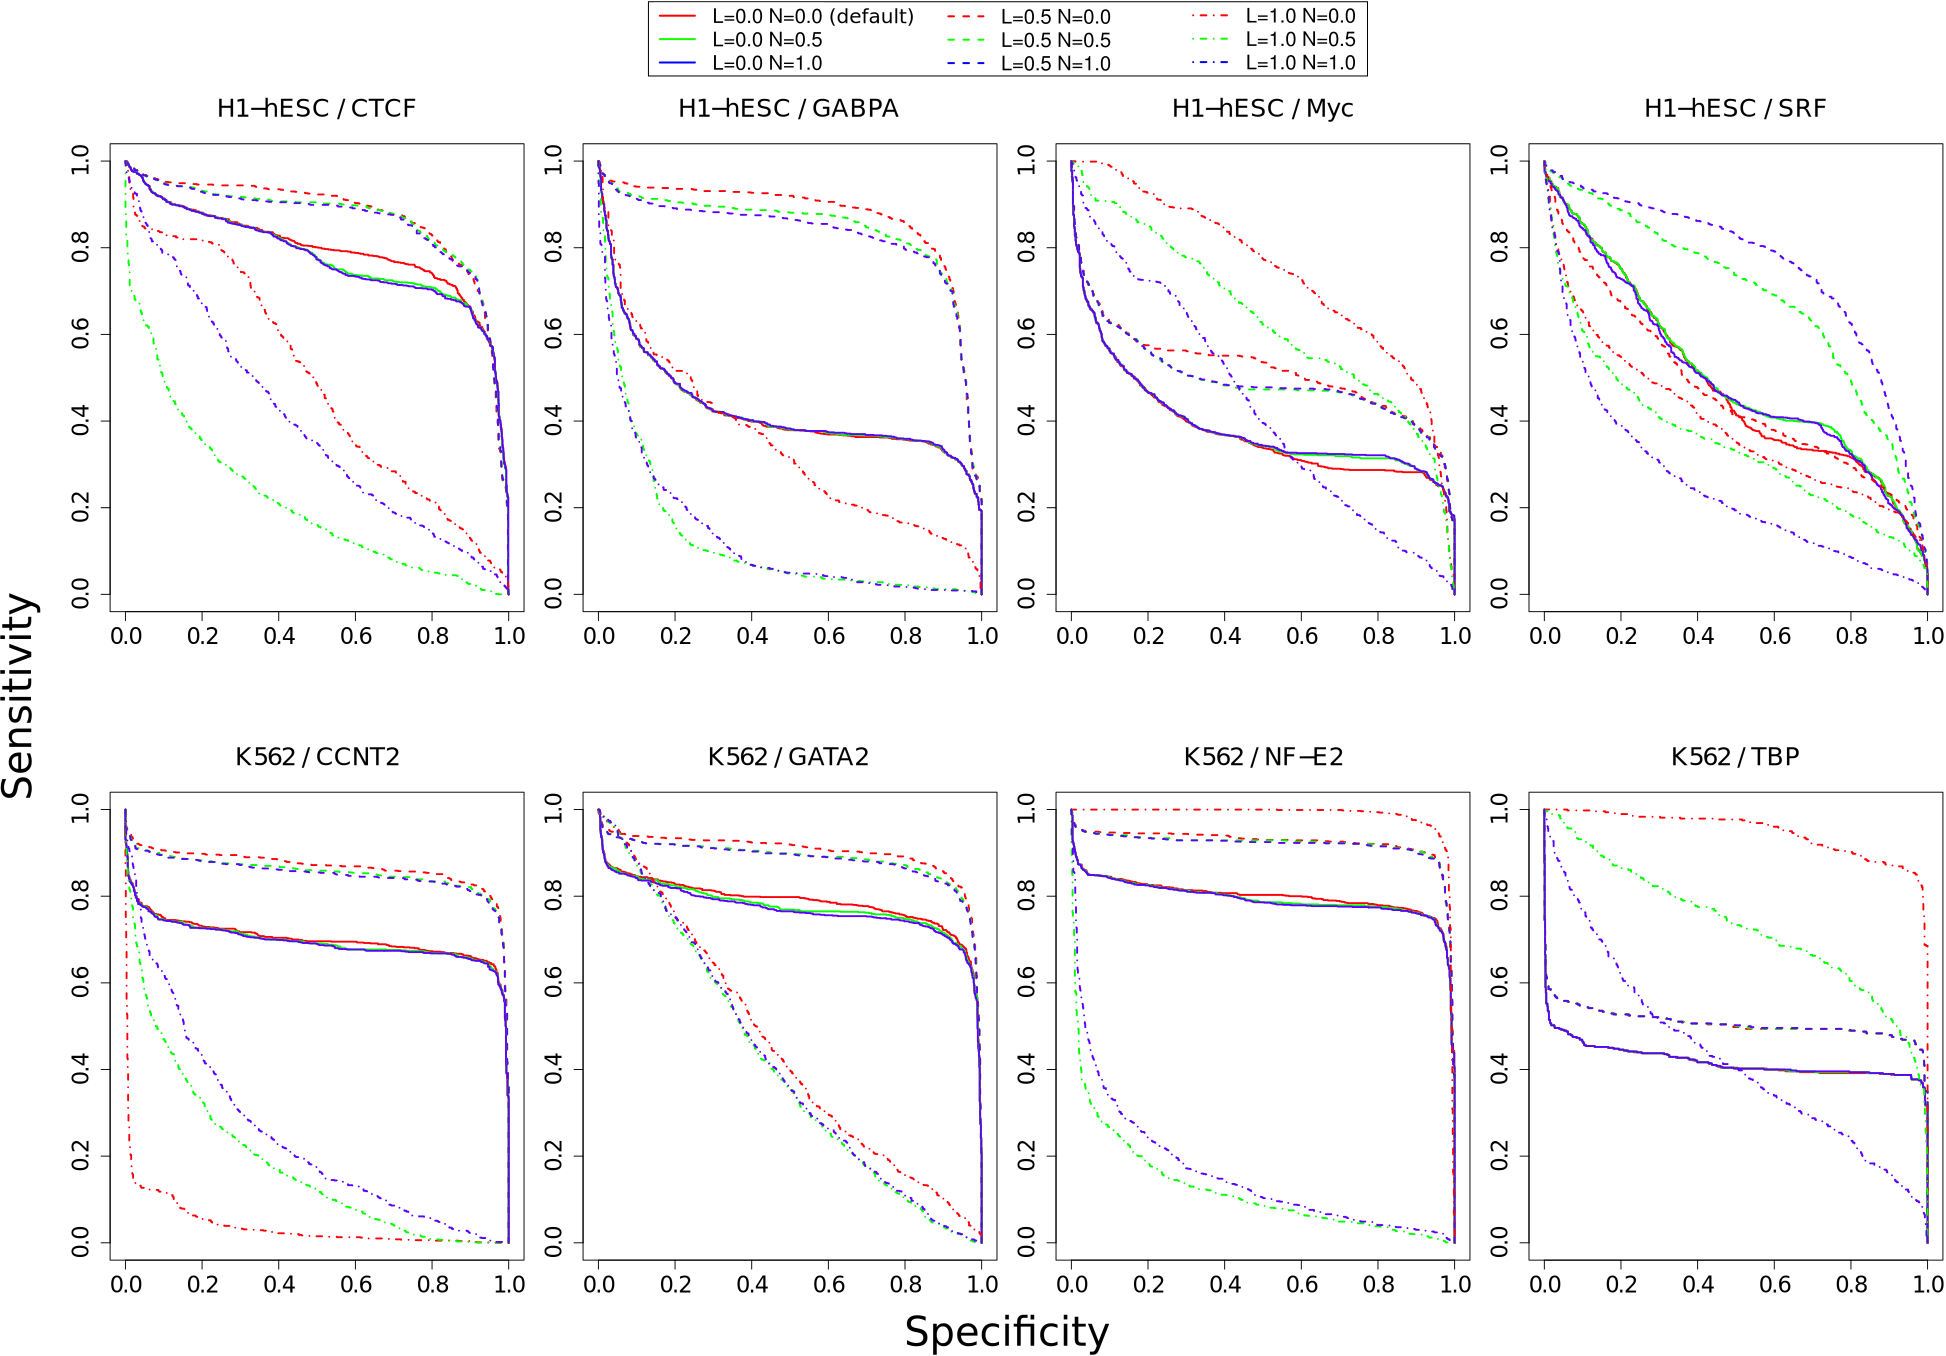
\includegraphics[width=0.99\textwidth]{gusmao_centipede_roc}
\caption[Centipede AUC variation]{\textbf{Centipede AUC variation.} Centipede's ROC curves created for multiple TFs based on a grid variation of Centipede's level of shrinkage of multinomial parameters ($L$) and level of shrinkage of negative binomial parameters ($N$) from $ 0.0 $ to $ 1.0 $ by $ 0.5 $.}
\label{fig:gusmao_centipede_roc}
\end{figure}

% Figure - Centipede parameter selection
\begin{figure}[h!]
\centering
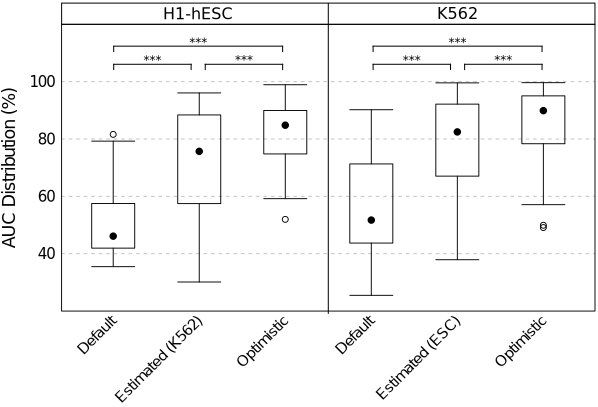
\includegraphics[width=0.99\textwidth]{gusmao_centipede_test}
\caption[Centipede parameter selection]{\textbf{Centipede parameter selection.} Distribution of AUCs for the three scenarios in which Centipede's level of shrinkage of multinomial parameters ($L$) and level of shrinkage of negative binomial parameters ($N$) were defined. `Default' refers to $L = N = 0.0$. `Estimated' refers to parameters estimated on a different cell type. `Optimistic' refers to parameters estimated on the same cell type for each TF individually. Statistical significance on the pairwise difference between these distributions is represented by the three-star system.}
\label{fig:gusmao_centipede_test}
\end{figure}

%%%%%%%%%%%%%%%%%%%%%%%%%%%%%%%%%%%%%%%%%%%%%%%%%%%%%%%%%%%%%%%%%%%%%
% Section: Cuellar Parameterization
%%%%%%%%%%%%%%%%%%%%%%%%%%%%%%%%%%%%%%%%%%%%%%%%%%%%%%%%%%%%%%%%%%%%%
\subsection{Cuellar Parameterization}
\label{sec:cuellar.parameterization}

To obtain Cuellar predictions, the program FIMO~\cite{grant2011} was used along with the priors, as suggested in Cuellar-Partida et al.~\ref{cuellar2012}. The establishment of the motif matching $p$-value threshold led to an issue similar to the selection of Centipede parameters (Section~\ref{sec:centipede.parameterization}), i.e. it was used a selection criteria based on \emph{a posteriori} evaluation of the AUCs obtained when using different FIMO $p$-value thresholds ($ 10^{-3} $, $ 10^{-4} $, $ 10^{-5} $, $ 10^{-6} $ and $ 10^{-7} $).

In Figure~\ref{fig:gusmao_cuellar_test} we can observe that the distribution of AUCs when FIMO $p$-value $ = 10^{-5}$ is used seems to outperforms all other thresholds. In order to test this claim, we performed a Friedman-Nemenyi test on the results of each FIMO $p$-value threshold. By observing the Friedman ranking and the Friedman-Nemenyi results available in Tables~\ref{tab:cuellarfimo.ranking} and~\ref{tab:cuellarfimo.fn.auc}, respectively, we are able to define the FIMO $p$-value $ = 10^{-5}$ as the best choice. Therefore, this value will be used in this study.

% Figure - Cuellar parameter selection
\begin{figure}[h!]
\centering
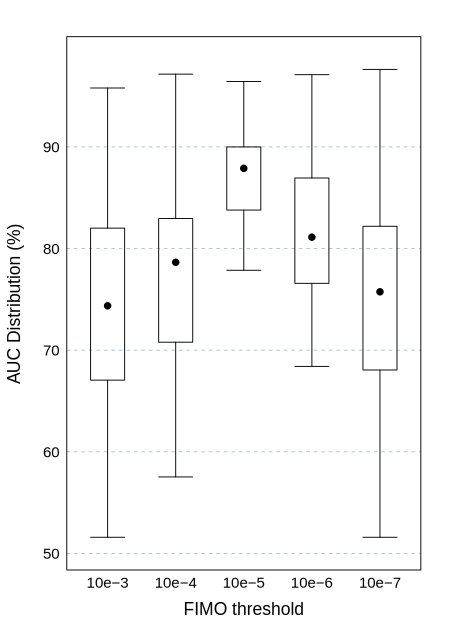
\includegraphics[width=0.99\textwidth]{gusmao_cuellar_test}
\caption[Cuellar parameter selection]{\textbf{Cuellar parameter selection.} Distribution of AUCs when using Cuellar's priors with different FIMO $p$-value thresholds.}
\label{fig:gusmao_cuellar_test}
\end{figure}

% Tables - Cuellar
% TODO

%%%%%%%%%%%%%%%%%%%%%%%%%%%%%%%%%%%%%%%%%%%%%%%%%%%%%%%%%%%%%%%%%%%%%
% Section: Conclusion
%%%%%%%%%%%%%%%%%%%%%%%%%%%%%%%%%%%%%%%%%%%%%%%%%%%%%%%%%%%%%%%%%%%%%
\section{Conclusion}
\label{sec:conclusion.5}

% Conclusion
In this chapter we justified the selection of parameters in multiple experimental features of this work. Parameter selection is indeed a very important set of analyses that should be present in all methodological studies in which the parameters impact on performance. Parameter selection should always consider two features: (1) the fairness of the approach, avoiding unrealistic optimal solutions; and (2) avoid data overfitting. The complexity of the experimental design presented here (different cells, methods and TFs) is justified by the considerations of both aforementioned features. Moreover, parameters which were not present in this chapter either do not impact significantly on the method's performance or have been previously described in other studies. Therefore, we did not include all the possible set of parameters for simplicity.


